\chapter{Load Balancer}

Il load balancing è una tecnica che consiste nella distribuzione del carico di lavoro tra molteplici server aumentando l'affidabilità a la scalabilità di un sistema. Nello specifico quello che verrà trattato in questo capitolo è il servizio LBaaS (Load Balancer as a Service) di OpenStack, ovvero il servizio di OpenStack che permette agli utenti di creare e utilizzare i load balancer.

I servizi di networking di OpenStack mettono a disposizione due diverse implementazioni di LBaaS attraverso il plugin \textit{neutron-lbaas}: LBaaS v1 (attualmente deprecato) e LBaaS v2. Octavia, il componente che è stato installato durante lo svolgimento di questo progetto, è una delle implementazioni di LBaaS v2.

Ci sono alcuni concetti e termini chiave riguardanti il funzionamento di Octavia e, più in generale, di LBaaS v2 che è necessario comprendere prima di proseguire con la descrizione dei componenti e dell'installazione; in \cref{fig:lbaas_schema} è presente il diagramma che rappresenta il funzionamento logico di LBaaS v2.

\begin{figure}[H]
    \center
    \includegraphics[scale=0.6]{tesi/files/immagini/lbaasv2-diagram.png}
    \caption{Diagramma concettuale di LBaaS v2 \cite{lbaas_docs}}
    \label{fig:lbaas_schema}
\end{figure}

\paragraph{Load Balancer.} Il load balancer occupa una porta di rete e ha un indirizzo IP assegnato da una subnet.

\paragraph{Listener.} I load balancer possono accettare richieste su porte multiple e supportano diversi tipi di protocolli. Il listener è l'elemento del load balancer che resta in ascolto su una determinata porta utilizzando un protocollo prestabilito e inoltra la richiesta al pool selezionato in fase di configurazione.

\paragraph{Pool.} Il pool è una lista di \emph{membri} che contiene tutte le informazioni riguardante l'algoritmo da utilizzare per il load balancing. All'interno del pool sono specificati anche il protocollo e la porta da utilizzare per accedere alle risorse esposte dai membri.

\paragraph{Members.} I membri sono server che forniscono le risorse richieste attraverso il load balancer. Ciascun membro è specificato dall'indirizzo IP e dalla porta che usa per fornire le risorse richieste; di conseguenza i membri possono essere macchine virtuali, container o server bare metal.

\paragraph{Health Monitor.} Gli health monitor servono per monitorare lo stato dei membri di un pool. Se ad esempio un macchina non è più raggiungibile per un qualsiasi motivo, l'health monitor se ne accorge e devia il traffico verso gli altri membri del pool. Gli health monitor sono associati ai pool.

\section{Componenti}

Nei capitoli seguenti verranno descritti i componenti di OpenStack che permettono la creazione di load balancer.%

\subsection{Octavia}

Octavia è una soluzione di load balancing open source progettata per lavorare insieme a OpenStack.

Octavia esegue i suoi compiti gestendo una flotta di macchine, container o server bare metal, noti comunemente come \textit{amphorae}, che vengono avviati su richiesta. Ciascuno di questi \textit{amphorae} contiene al suo interno un'istanza di load balancer \cite{octavia_docs}.

\subsection{Barbican}

Barbican è il Key Manager di OpenStack, ovvero il servizio che si occupa di memorizzare e gestire i dati segreti, come ad esempio chiavi simmetriche, chiavi asimmetriche, certificati, password e dati binari \cite{barbican_docs}. Come si può intuire, le sue funzionalità sono molto simili a quelle di Vault (descritto nel capitolo \ref{sec:vault}), però è necessario installare anche Barbican perché Octavia non ha un supporto diretto per Vault. È possibile però configurare Barbican in modo che utilizzi Vault come backend, in modo da avere una gestione unificata di tutti i \textit{secrets}.



\section{Installazione}

\subsection{Installazione manuale}

Le istruzioni per l'installazione riportate in questo capitolo danno come presupposto che si disponga di un cloud OpenStack base già installato e funzionante.

\paragraph{Barbican.} Il primo passo è installare i charm barbican e barbican-vault, che sono rispettivamente Barbican e il software che permette l'integrazione tra Barbican e Vault con le rispettive relazioni:
\begin{lstlisting}[language=mybash]
juju deploy barbican --channel yoga/stable --series focal --to lxd:3
juju deploy barbican-vault --channel yoga/stable --series focal
juju add-relation barbican rabbitmq-server
juju add-relation barbican keystone
juju add-relation barbican barbican-vault
juju add-relation barbican-vault:secrets barbican:secrets
juju add-relation vault:secrets barbican-vault:secrets-storage
\end{lstlisting}
Il secondo passo è installare un router MySQL per permettere a Barbican di collegarsi al cluster InnoDB e aggiungere le relazioni necessarie:
\begin{lstlisting}[language=mybash]
juju deploy mysql-router barbican-mysql-router --channel 8.0/stable --series focal
juju add-relation barbican-mysql-router:db-router mysql-innodb-cluster:db-router
juju add-relation barbican-mysql-router:shared-db barbican:shared-db
\end{lstlisting}

\paragraph{Octavia.} Dopo l'installazione di Barbican si può procedere con quella di Octavia. Prima di procedere con l'installazione vera e propria è necessario però riconfigurare Neutron per abilitare il driver per l'estensione ML2. È necessario fare questo perché i gruppi di sicurezza di OpenStack hanno delle policy anti-spoofing che non permettono alle macchine virtuali di instradare il traffico attraverso loro stesse e, grazie a questa estensione, è possibile specificare dei flag che permettono di abilitare o disabilitare i filtri sulle porte \cite{neutron_ml2_docs}. Per abilitare l'estensione ML2 è necessario eseguire il seguente comando:
\begin{lstlisting}[language=mybash]
juju config neutron-api enable-ml2-port-security=True
\end{lstlisting}
Fatto questo si può procedere con l'installazione di Octavia:
\begin{lstlisting}[language=mybash]
juju deploy octavia --channel yoga/stable --series focal --to lxd:3
juju add-relation octavia rabbitmq-server
juju add-relation octavia keystone
juju add-relation octavia:neutron-openvswitch ovn-chassis:nova-compute
juju add-relation octavia neutron-api
\end{lstlisting}
Successivamente si può installare il router MySQL che permette la connessione al cluster InnoDB con le relative relazioni:
\begin{lstlisting}[language=mybash]
juju deploy mysql-router octavia-mysql-router --channel 8.0/stable --series focal
juju add-relation octavia-mysql-router:db-router mysql-innodb-cluster:db-router
juju add-relation octavia-mysql-router:shared-db octavia:shared-db
\end{lstlisting}
Infine è necessario installare Octavia Dashboard, il plugin per OpenStack Dashboard che mette a disposizione l'interfaccia grafica per configurare i load balancer:
\begin{lstlisting}[language=mybash]
juju deploy octavia-dashboard --channel yoga/stable --series focal
juju add-relation octavia-dashboard openstack-dashboard
\end{lstlisting}

\subsection{Installazione in bundle}

L'installazione in bundle prevede l'utilizzo di un file bundle analogo a quello visto nella \cref{sec:openstack_installazione_bundle} riguardante l'installazione di OpenStack, con l'unica differenza che in questo caso il bundle è stato strutturato come overlay (per ulteriori dettagli vedere la \cref{subsec:juju_concetti}).
È stata presa questa decisione per 2 motivi:
\begin{enumerate}
    \item il load balancer non è un componente necessario per far funzionare OpenStack, quindi creando un overlay su può decidere se installarlo o meno
    \item durante lo svolgimento del progetto l'installazione del load balancer è stata fatta successivamente alla prima installazione di OpenStack, quindi con un overlay è stato possibile eseguire un'installazione tramite bundle senza dover eliminare e ricreare il cloud già esistente
\end{enumerate}

Utilizzando un overlay per il deployment ci si può trovare in due situazioni:
\begin{enumerate}
    \item deve essere installato tutto il sistema (compreso il bundle principale)
    \item si deve installare solo l'overlay su un sistema già esistente
\end{enumerate}

Nel caso in cui si debba installare tutto il sistema sarà sufficiente eseguire il deployment del bundle aggiungendo l'opzione \verb|--overlay| e specificando il nome del bundle overlay come nell'esempio seguente:
\begin{lstlisting}[language=mybash]
juju deploy ./bundle.yaml --overlay ./overlays/octavia.yaml
\end{lstlisting}

Nel caso in cui si voglia aggiungere l'overlay ad un'installazione già esistente sarà necessario esportare il modello di Juju in un file bundle e poi eseguire il deploy del modello aggiungendo l'overlay. Di seguito è riportato un esempio:
\begin{lstlisting}[language=mybash]
juju export-bundle --filename exported-bundle.yaml
juju deploy ./exported-bundle.yaml --overlay ./overlays/octavia.yaml
\end{lstlisting}

\section{Configurazione iniziale}

Il primo passo per configurare il load balancer di OpenStack è generare i certificate necessari per l'autenticazione e la comunicazione sicura tra gli \emph{Amphorae} (le istanze del load balancer) e il sistema di controllo di Octavia \cite{load_balancer_installation_guide}. Per fare questo è necessario eseguire i seguenti comandi:
\begin{lstlisting}[language=mybash]
mkdir -p demoCA/newcerts
touch demoCA/index.txt
touch demoCA/index.txt.attr

openssl genpkey -algorithm RSA -aes256 -pass pass:foobar -out issuing_ca_key.pem
openssl req -x509 -passin pass:foobar -new -nodes -key issuing_ca_key.pem \
    -config /etc/ssl/openssl.cnf \
    -subj "/C=US/ST=Somestate/O=Org/CN=www.example.com" \
    -days 365 \
    -out issuing_ca.pem

openssl genpkey -algorithm RSA -aes256 -pass pass:foobar -out controller_ca_key.pem
openssl req -x509 -passin pass:foobar -new -nodes \
        -key controller_ca_key.pem \
    -config /etc/ssl/openssl.cnf \
    -subj "/C=US/ST=Somestate/O=Org/CN=www.example.com" \
    -days 365 \
    -out controller_ca.pem
openssl req \
    -newkey rsa:2048 -nodes -keyout controller_key.pem \
    -subj "/C=US/ST=Somestate/O=Org/CN=www.example.com" \
    -out controller.csr
openssl ca -passin pass:foobar -config /etc/ssl/openssl.cnf \
    -cert controller_ca.pem -keyfile controller_ca_key.pem \
    -create_serial -batch \
    -in controller.csr -days 365 -out controller_cert.pem
cat controller_cert.pem controller_key.pem > controller_cert_bundle.pem
\end{lstlisting}

Successivamente si deve configurare il charm con i certificati appena generati. Per fare questo è sufficiente eseguire il seguente comando:
\begin{lstlisting}[language=mybash]
juju config octavia \
    lb-mgmt-issuing-cacert="$(base64 issuing_ca.pem)" \
    lb-mgmt-issuing-ca-private-key="$(base64 issuing_ca_key.pem)" \
    lb-mgmt-issuing-ca-key-passphrase=foobar \
    lb-mgmt-controller-cacert="$(base64 controller_ca.pem)" \
    lb-mgmt-controller-cert="$(base64 controller_cert_bundle.pem)"
\end{lstlisting}

Per completare la configurazione e l'attivazione di Octavia è necessario configurare le risorse (reti e macchine virtuali) che dovrà utilizzare. Dato che la gestione delle risorse di Octavia è automatizzata, per svolgere quest'ultima operazione è sufficiente eseguire il seguente comando:
\begin{lstlisting}[language=mybash]
juju run-action --wait octavia/0 configure-resources
\end{lstlisting}

Come detto in precedenza Octavia utilizza una serie di macchine virtuali gestite in maniera automatica per istanziare i load balancer; di conseguenza è necessario anche fornire delle immagini di sistemi operativi che possano essere utilizzate per queste macchine virtuali. È possibile scaricare e importare queste immagini automaticamente eseguendo i seguenti comandi:
\begin{lstlisting}[language=mybash]
juju run-action --wait glance-simplestreams-sync/0 sync-images
juju run-action --wait octavia-diskimage-retrofit/leader retrofit-image
\end{lstlisting}

\section{Utilizzo}

Prima di poter utilizzare le funzionalità messe a disposizione dal load balancer è necessario assicurarsi che l'utente che si sta utilizzando abbia i permessi per accedere a queste funzionalità; Octavia infatti crea in maniera automatica alcuni ruoli che possono essere utilizzati per garantire diversi tipi di accesso e di privilegi agli utenti. I ruoli sono i seguenti:

\begin{itemize}
    \item \textbf{load-balancer\_observer}: garantisce privilegi di sola lettura
    \item \textbf{load-balancer\_global\_observer}: garantisce privilegi di sola lettura estesi anche a risorse appartenenti ad altri utenti
    \item \textbf{load-balancer\_member}: garantisce privilegi di lettura e scrittura sul load balancer
    \item \textbf{load-balancer\_quota\_admin}: garantisce privilegi di amministrazione solamente sulle quota API, ovvero sulle API che permettono di impostare il massimo numero di risorse utilizzabili da un utente o da un progetto
    \item \textbf{load-balancer\_admin}: garantisce privilegi di amministrazione su tutte le risorse di load balancing, incluse quelle appartenenti ad altri utenti
\end{itemize}

Per poter aggiungere uno di questi ruoli ad un utente è sufficiente eseguire il seguente comando:
\begin{lstlisting}[language=mybash]
openstack role add --user-domain domain1 --user user1 \
   --project-domain domain1 --project project1 \
   load-balancer_member
\end{lstlisting}

\subsection{Creazione di un load balancer}

Tutte le operazioni riguardanti i load balancer possono essere eseguite tramite la pagina raggiungibile dal menu a tendina \emph{Project} > \emph{Network} selezionando la voce \emph{Load Balancers}.

\begin{figure}[H]
    \center
    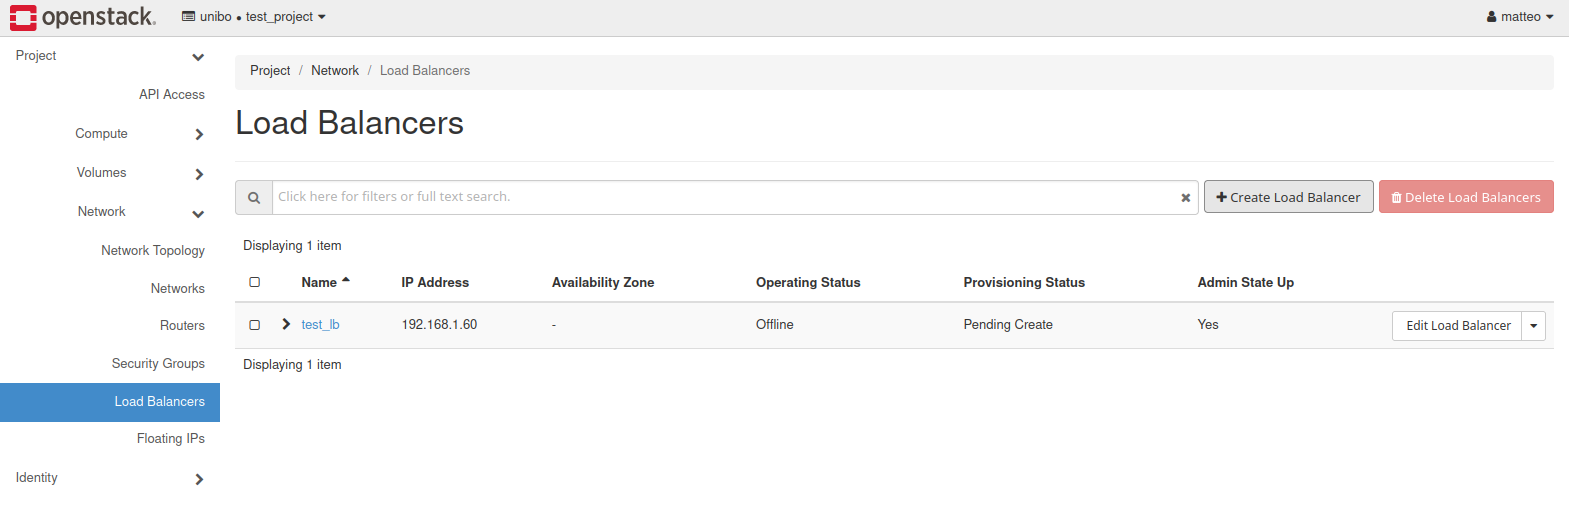
\includegraphics[scale=0.35]{tesi/files/immagini/load_balancer_usage/load_balancers_interface.png}
    \caption{Interfaccia di gestione dei load balancers}
    \label{fig:lb_mgmt_interface}
\end{figure}

Per creare un nuovo load balancer si deve cliccare il bottone \emph{Create load balancer}; in questo modo verrà aperta una finestra di dialogo che consentirà all'utente di inserire tutti i parametri di configurazione. Gli unici parametri obbligatori sono il nome e la subnet alla quale collegare l'interfaccia di rete. È possibile inoltre creare il listener e il pool direttamente da questa finestra di dialogo, però questi elementi verranno trattati nella \cref{subsec:load_balancer_management}.

\subsection{Gestione del load balancer}\label{subsec:load_balancer_management}

Cliccando sul nome di uno dei load balancer è possibile accedere alla pagina di gestione, dalla quale si possono visualizzare tutte le informazioni riguardanti il load balancer selezionato e gestire i listener e i pool.

\begin{figure}[H]
    \center
    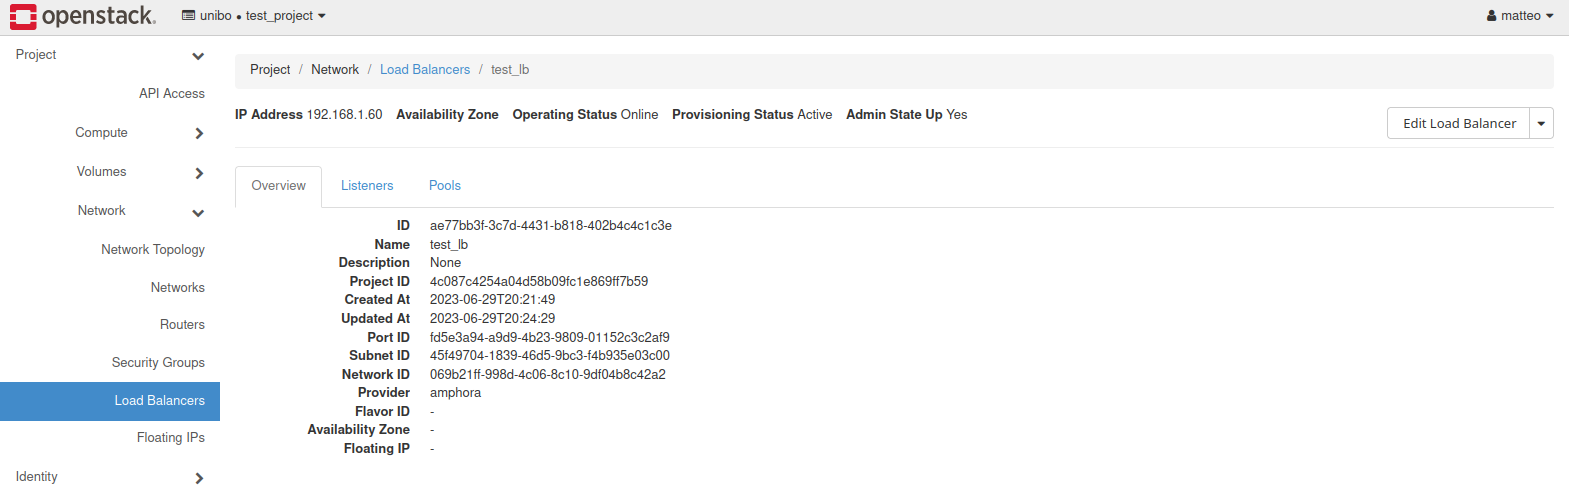
\includegraphics[scale=0.35]{tesi/files/immagini/load_balancer_usage/load_balancer_settings.png}
    \caption{Interfaccia configurazione di un load balancer}
    \label{fig:lb_settings}
\end{figure}

\paragraph{Listener.} È possibile aggiungere e modificare i listener dall'interfaccia di configurazione del load balancer andando nella scheda \emph{Listeners}. Per creare un nuovo listener si vede cliccare sul bottone \emph{Create Listener} e inserire tutti i parametri di configurazione richiesti. Nello specifico i parametri sono i seguenti:
\begin{itemize}
    \item \textbf{Name}: nome del listener
    \item \textbf{Protocol}: protocollo su cui il listener resta in ascolto
    \item \textbf{Port}: porta sulla quale il listener resta in ascolto
    \item \textbf{Client Data Timeout}: timeout del client (espresso in millisecondi)
    \item \textbf{TCP Inspect Timeout}: tempo massimo di attesa di ulteriori pacchetti TCP per l'ispezione del contenuto
    \item \textbf{Member Connect Timeout}: timeout di connessione per i membri dei pool
    \item \textbf{Member Data Timeout}: timout di inattività per i membri dei pool
    \item \textbf{Connection Limit}: numero massimo di connessioni simultanee (si può disabilitare inserendo -1)
    \item \textbf{Allowed Cidrs}: permette di restringere le connessioni solamente alle subnet specificate
\end{itemize}

È possibile inoltre creare un pool contemporaneamente al listener oppure associarene uno in seguito.

\paragraph{Pool.} Per creare e gestire i pool si deve aprire la scheda \emph{Pools} all'interno dell'interfaccia di gestione del load balancer. Da qui è possibile midificare o pool esistenti oppure crearne uno nuovo cliccando sul bottone \emph{Create Pool}. I parametri richiesti per la creazione di un nuovo pool sono:
\begin{itemize}
    \item \textbf{Name}: nome del pool
    \item \textbf{Algorithm}: algoritmo da utilizzare per il load balancing (tutti gli algoritmi sono descritti nel paragrafo seguente)
    \item \textbf{Protocol}: protocollo utilizzato dai membri del pool
    \item \textbf{Session Persistance}: permette di indicare il tipo di persistenza della sessione da utilizzare
    \item \textbf{TLS Enabled}: se attivato le connessioni tra il load balancer e i membri vengono cifrate
\end{itemize}

\paragraph{Algoritmi di load balancing.}
Il load balancer utilizzato durante lo svolgimento di questo progetto implementa 3 diversi algoritmi di load balancing:
\begin{itemize}
    \item Least Connections
    \item Round Robin
    \item Source IP
\end{itemize}

L'algoritmo \emph{Least Connections} inoltra la richiesta del client al membro del pool con il minor numero di connessioni attive al momento della richiesta. Questo può essere molto utile nel caso in cui le richieste all'applicazione ospitata dietro il load balancer abbiano tempi di risposta molto diversi (ad esempio il download di file) e nel caso in cui tutti i membri del pool abbiano risorse hardware molto simili.

L'algoritmo \emph{Round Robin} inoltra le richieste dei client a rotazione a tutti i membri del pool. Questo algoritmo può essere molto utile in casi in cui tutte le richieste sono molto simili come tempi di risposta e complessità delle operazioni da eseguire, ma potrebbe essere inefficiente nel caso in cui le richieste hanno tempi di risposta molto diversi o richiedono l'esecuzione di calcoli molto complessi.

L'algoritmo \emph{Source IP} consiste nell'indirizzare tutte le richieste provenienti dallo stesso indirizzo IP al medesimo membro del pool. Questo algoritmo è utile specialmente quando è imperativo che il client si connetta sempre allo stesso server per ciascuna richiesta.


\paragraph{Tipi di persistenza della sessione.}
Octavia implementa 3 tecniche di persistenza della sessione:
\begin{itemize}
    \item Source IP
    \item HTTP Cookie
    \item APP Cookie
\end{itemize}

Come si può intuire, se si utilizza la tecnica \emph{Source IP} la sessione viene mantenuta in base all'indirizzo IP del client. Utilizzando invece la tecnica \emph{HTTP Cookie} viene generato in automatico un cookie HTTP aggiuntivo che permette al load balancer di capire a quale membro del pool il client si è connesso in precedenza. La tecnica \emph{APP Cookie} è molto simile come funzionamento alla precedente, con l'unica differenza che il cookie non viene generato in automatico ma viene impostato dall'applicazione ospitata dietro il load balancer e, durante la configurazione del pool, deve essere specificato qual è il nome di questo cookie.

